\section{Ziel}
\label{sec:Ziel}
Durch diesem Versuch werden die fundamentalen physikalischen Gesetze der Strahlenoptik untersucht. Dazu wird überprüft, ob sich monochromatisches Licht unter Beugung, Brechung 
und Reflexion der Theorie nach verhält.

\section{Theorie}
\label{sec:Theorie}
Licht ist eine elektromagnetische Welle. Daher kann Licht in komplexer Weise durch die Maxwell-Gleichungen beschrieben werden. Dies ist für die fundamentalen Gesetze der
Strahlenoptik nicht nötig. Es genügt Licht auf ein einfacheres Verhalten zu vereinfachen. Dazu wird Licht ,aufbauend auf den niederländischen Physiker 
\textit{Christiaan Huygens}, auf das Ausbreitungsverhalten reduziert. Gemäß des \textit{Huygensschen Prinzips} breitet sich Licht entlang der Wellennormalen aus. Die 
Wellennormale steht immer orthogonal zur \textit{Wellenfront} und ist in \autoref{fig:Huygensbrechung} durch einen roten Pfeil skizziert. Das Huygenssche Prinzip sagt nun aus,
dass sich die Welle ausbreitet indem an jedem Punkt der Wellenfront eine neue radiale Elementarwelle entsteht. Durch Überlagerung aller dieser Elementarwellen ergibt sich 
eine neue Wellenfront. Dies beschreibt eine gradlinige Propagation einer Lichtwelle ohne Veränderung des Ausbreitungsmediums. Trifft eine Welle mit diesem gedanklichem Modell
nun auf ein unterschiedliches Medium wird die Welle \textit{gebrochen},\textit{gebeugt} und oder \textit{reflektiert}. Diese Wechselwirkung mit einem anderem Medium entsteht, 
da sich Wellen, so auch die Elementarwellen nach Huygens, in unterschiedlichen Medien unterschiedlich schnell ausbreiten. Die drei genannten Wechselwirkungen treten dann in 
Abhänigkeit vom Licht und Beugungsmaterial auf. 

\begin{figure}
    \centering
    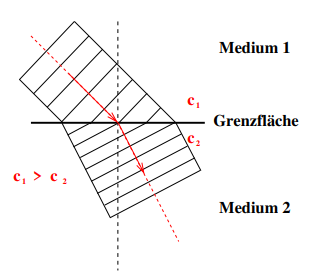
\includegraphics[width=0.5\textwidth]{content/HuygensscheBrechung.png}
    \caption{In dieser Abbildung ist schematisch das Huygenssche Prinzip dargestellt. \cite{v400}.}
    \label{fig:Huygensbrechung}
  \end{figure}

\subsection{Reflexion}
\label{subsec:reflexion}
